\documentclass{article}

\usepackage{tikz}
\usepackage{geometry}
\usetikzlibrary{positioning}
\geometry{left=1.0cm} 
\usetikzlibrary{automata,positioning,arrows,chains,shapes}

\begin{document}

	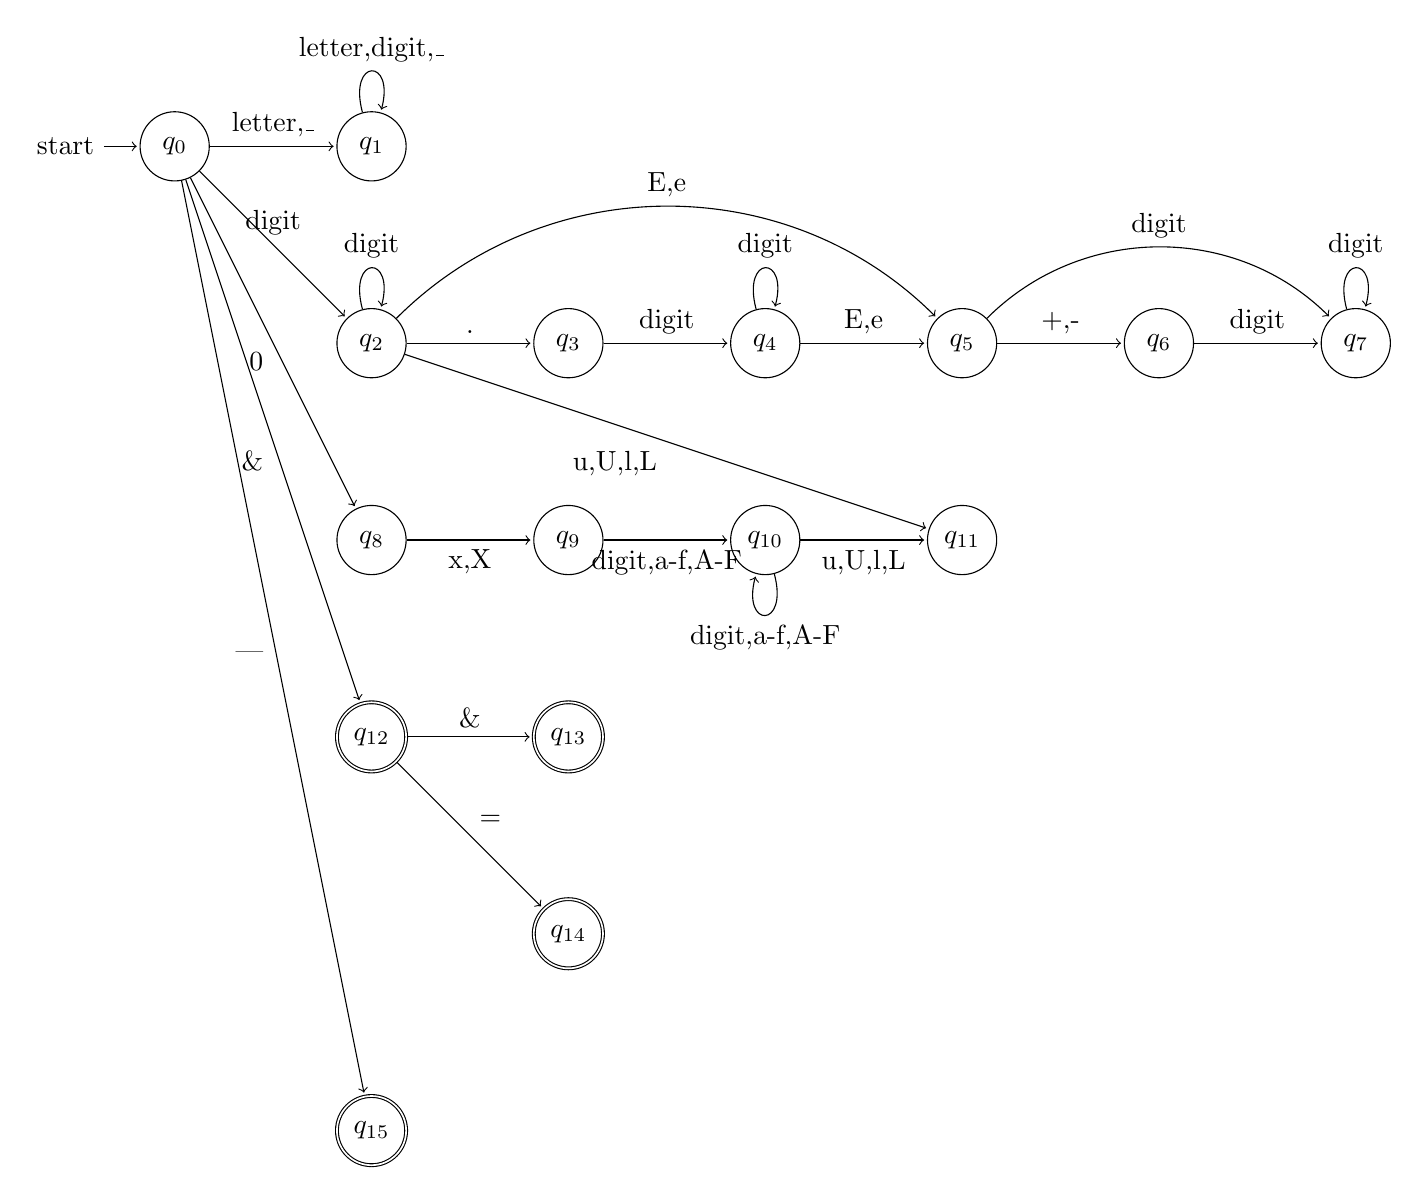
\begin{tikzpicture}[shorten >=1pt,node distance=2.5cm,on grid,auto] 
		\node[state,initial] (q_0)   {$q_0$}; 
		\node[state] (q_1) [right=of q_0] {$q_1$}; 
		\node[state] (q_2) [below=of q_1] {$q_2$}; 
		\node[state] (q_3) [right=of q_2] {$q_3$}; 
		\node[state] (q_4) [right=of q_3] {$q_4$}; 
		\node[state] (q_5) [right=of q_4] {$q_5$}; 
		\node[state] (q_6) [right=of q_5] {$q_6$}; 
		\node[state] (q_7) [right=of q_6] {$q_7$}; 
		\node[state] (q_8)[below=of q_2]  {$q_8$}; 
		\node[state] (q_9)[right=of q_8]  {$q_9$};
		
		\node[state] (q_10)[right=of q_9]  {$q_{10}$};  
		\node[state] (q_11)[right=of q_10]  {$q_{11}$};  
		
		\node[state,accepting] (q_12)[below=of q_8]  {$q_{12}$}; 
		\node[state,accepting] (q_13)[right=of q_12]  {$q_{13}$};
		\node[state,accepting] (q_14)[below=of q_13]  {$q_{14}$};
		
		\node[state,accepting] (q_15)[below =5cm of q_12]  {$q_{15}$};
%		\node[state,accepting](q_final) [below right=of q_1] {$FINAL$};
		\path[->] 
		(q_0) edge  node {letter,\_} (q_1)
		edge  node [above] {digit} (q_2)
		edge  node [swap] {0} (q_8)
		edge  node [swap] {\&} (q_12)
		edge  node [swap] {|} (q_15)
		(q_1) edge  [loop above] node {letter,digit,\_} ()
		(q_2) edge  node {.} (q_3)
		      edge  [loop above] node {digit} ()
		      edge  [bend left=45] node {E,e} (q_5)
		      edge  [swap] node {u,U,l,L} (q_11)
		(q_3) edge  node {digit} (q_4)
		(q_4) edge  node {E,e} (q_5)
	          edge  [loop above] node {digit} ()
		(q_5) edge  node {+,-} (q_6)
			edge  [bend left=45] node {digit} (q_7)
		(q_6) edge  node {digit} (q_7)
		(q_7) edge  [loop above] node {digit} ()
		(q_8)  edge  node [swap] {x,X} (q_9)
		(q_9) edge  [swap] node {digit,a-f,A-F} (q_10)
		(q_10) edge  [loop below] node {digit,a-f,A-F} ()
			 edge  [swap] node {u,U,l,L} (q_11)
		(q_12) edge  node {\&} (q_13)
		(q_12) edge  node {=} (q_14)
	%	(q_2) edge  node [swap] {0} (q_final);
		%edge [loop below] node {1} ();
		;
	\end{tikzpicture}

\end{document}  